\documentclass[border={1cm 1cm 1cm 1cm}]{standalone}

\usepackage{tikz}
\usetikzlibrary{calc}	%for centerarc

\def\centerarc[#1](#2)(#3:#4:#5)
{ \draw[#1] ($(#2)+({#5*cos(#3)},{#5*sin(#3)})$) arc (#3:#4:#5); }

%“Spinoza's universe,” from Lord, B. (2010). Spinoza's Ethics. Edinburgh University Press, p. 41

\begin{document}
	
	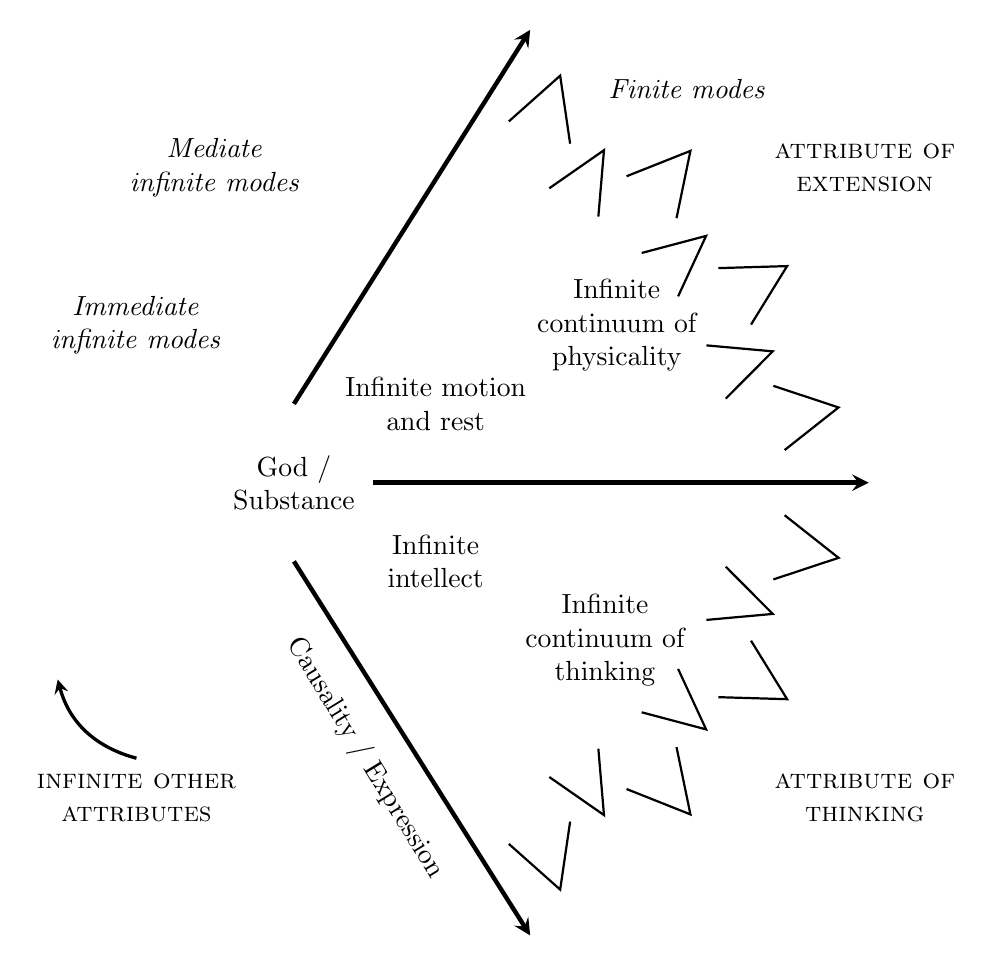
\begin{tikzpicture}	
	%ARCS
	\centerarc[very thick,gray](0,0)(-100:100:1)
	\centerarc[very thick,gray](0.5,0)(-80:85:3)
	\centerarc[very thick,gray](1.5,0)(-83:100:5)
	
	%ARROWS
	%from center
	\draw[ultra thick,->,>=stealth] (1, 0)--(7.3, 0);
	\draw[ultra thick,->,>=stealth] (0, 1)--(3, 5.75);
	\draw[ultra thick,->,>=stealth] (0,-1)--(3,-5.75);
	%bottom left
	\draw[very thick,->,>=stealth] (-2,-3.5) to[bend left] (-3,-2.5);
	
	%LABELS
	\node[align=center] at (0,0)	 {God /\\ Substance};
	\node[align=center] at (1.8, 1)  {Infinite motion\\ and rest};
	\node[align=center] at (1.8,-1)  {Infinite\\ intellect};
	\node[align=center] at (4.1, 2)  {Infinite\\ continuum of\\physicality};
	\node[align=center] at (3.95,-2) {Infinite\\continuum of\\thinking};
	\node[align=center] at (.9,-3.5) {\rotatebox{-58.5}{Causality / Expression}};
	\node[align=center] at (-2,-4)	 {\textsc{infinite other}\\\textsc{attributes}};
	\node[align=center] at (7.25,4)	 {\textsc{attribute of}\\\textsc{extension}};
	\node[align=center] at (7.25,-4) {\textsc{attribute of}\\\textsc{thinking}};
	\node[align=center] at (-2,2)	 {\textit{Immediate}\\\textit{infinite modes}};
	\node[align=center] at (-1,4)	 {\textit{Mediate}\\\textit{infinite modes}};
	\node[align=center] at (5,5)	 {\textit{Finite modes}};
	
	%SPIKES
	\foreach \x in {0,...,7}{ 		%outer spikes
	\centerarc[line width=1.7,white](1.5,0)({66.8-20*\x}:{73.2-20*\x}:5)	%cover grey circle
	\draw[thick] ({1.5+4.75*cos(75-20*\x)},{4.75*sin(75-20*\x)}) -- 
				 ({1.5+5.5*cos(70-20*\x)},{5.5*sin(70-20*\x)}) -- 
				 ({1.5+4.75*cos(65-20*\x)},{4.75*sin(65-20*\x)});
		}
	\foreach \x in {0,1,2,4,5,6} 	%inner spikes (missing 3 b/c overlaps with arrow)
	\draw[thick] ({1.5+4.125*cos(65-20*\x)},{4.125*sin(65-20*\x)}) -- 
				 ({1.5+4.875*cos(60-20*\x)},{4.875*sin(60-20*\x)}) -- 
				 ({1.5+4.125*cos(55-20*\x)},{4.125*sin(55-20*\x)});
	
%	\centerarc[red](1.5,0)(-83:100:4.5)		\centerarc[red](1.5,0)(-83:100:4.75)
%	\centerarc[red](1.5,0)(-83:100:5.25)	\centerarc[red](1.5,0)(-83:100:5.5)
%	\draw[help lines] (-2,-5) grid (8,7);
	\end{tikzpicture}
	
\end{document}